\documentclass[11pt,fleqn]{article}
%\usepackage{CJK}
\usepackage{latexsym}
\usepackage{color}
\usepackage{graphicx, float}\usepackage{graphicx}
%\usepackage{algorithmicx}
\usepackage{algorithm}
\usepackage{algpseudocode}
%\usepackage[colorlinks]{hyperref}
\setlength{\oddsidemargin}{-0.0in}
\setlength{\evensidemargin}{-0.0in} \setlength{\textwidth}{6.0in}
\setlength{\textheight}{9.0in} \setlength{\topmargin}{-0.2in}

%\setlength{\leftmargin}{0.7in}
\usepackage{amssymb, graphicx, amsmath}  %  fancyheadings,
\usepackage{setspace}
\newcommand\qed{\qquad $\square$}
\newcommand{\nn}{\nonumber}

\def \[{\begin{equation}}
\def \]{\end{equation}}
\def\proof{{\bf Proof:\quad}}
\def \endzm {\quad $\Box$}
\def\dist{\hbox{dist}}


\newcommand{\R}{\mathbb{R}}
%\newtheorem{yinli}{����}[section]
\newcommand{\D}{\displaystyle}
\newcommand{\T}{\textstyle}
\newcommand{\SC}{\scriptstyle}
\newcommand{\FT}{\footnotesize}



%\newtheorem{theorem}{Theorem}[section]
%\renewcommand{\thetheorem}{\arabic{section}.\arabic{theorem}}
\newtheorem{definition}{Definition}
\renewcommand{\thedefinition}{\arabic{section}.\arabic{definition}}
\newtheorem{lemma}{Lemma}[section]
\renewcommand{\thelemma}{\arabic{section}.\arabic{lemma}}
\newtheorem{remark}{Remark}
\renewcommand{\theremark}{\arabic{section}.\arabic{remark}}
\newtheorem{proposition}{Proposition}[section]
\renewcommand{\theproposition}{\arabic{section}.\arabic{proposition}}
\newtheorem{corollary}{Corollary }[section]
\renewcommand{\thecorollary}{\arabic{section}.\arabic{corollary}}
\renewcommand{\theequation}{\arabic{section}.\arabic{equation}}
\renewcommand{\baselinestretch}{1.35}
\newtheorem{exam}{Example}[section]
\renewcommand{\theexam}{\arabic{section}.\arabic{exam}}
\newtheorem{theo}{Theorem}[section]
\renewcommand{\thetheo}{\arabic{section}.\arabic{theo}}
\begin{document}
%\begin{CJK*}{GBK}{song}

\begin{center}

{\LARGE \bf  Machine Learning Assignment 2}\\


\vskip 25pt
 {Huihuang Zheng, huihuang@utexas.edu }\\
\vskip 5pt
{\small hz4674 Spring 2016 }

\end{center}

\begin{spacing}{1.5}
\section{Using Code}
To run my code, open \textbf{src/main.m}, change the \textbf{DATA\_DIR} to where you put your \textbf{icatest.mat} and \textbf{sounds.mat}, then run the \emph{src/main.m} with Matlab. It will output one figure of mixed signals and one figure which put origin signals and estimated signals together. For comparison of origin signals and estimated signals, those signals are listed in $n$ rows and 2 columns, where $n$ is the number of signals. The order may not be correct. But you can find the matched shape.

\section{Algorithm Implementation}

The \textbf{src/mixSignals.m} mixes source signals for inputs of source signals and mixing matrix. If you don't specify a mixing matrix, I generate a random one. The \textbf{src/ICA.m}) is the function calculating recovered signals and unmixing matrix. Other functions {src/rescaleVector.m} {src/showResult.m} and {src/showSignal.m} are just used for printing results. My algorithm is exactly same as on Canvas assignment page. But I change something about the learning rate. In website page, it suggested that when we deal with the large data set \textbf{sounds.mat}, our program may be slow, then we can set smaller learning step. Let our unmixing matrix in $i$-th iteration be $W_i$. Let the norm of difference of unmixing matrices in two neighbor iteration, which is $norm(W_{i} - W_{i-1})$ be $\Delta$. Let the converge threshold be $H$, then the algorithm stops when $\Delta < H$. In my experiment, I found when we set smaller learning rate, it still converge slow (about ten thousands of iterations if I set $H = 1e^{-9}$). I did this in different way: I set a large learning rate, but after a number of iterations, I decrease the learning rate, which makes converge faster than smaller learning rate at beginning and can converge with smaller learning rate at the end. I set initial learning rate to 0.1 and for every 1000 iterations, I multiply learning rate by 0.1. Be doing so, my program just converge at thousands of iterations.

\section{Experiment}
\subsection{Small Dataset}
I run experiment using \textbf{icatest.mat}. My program runs pretty well in this dataset. See result:
\begin{center}
    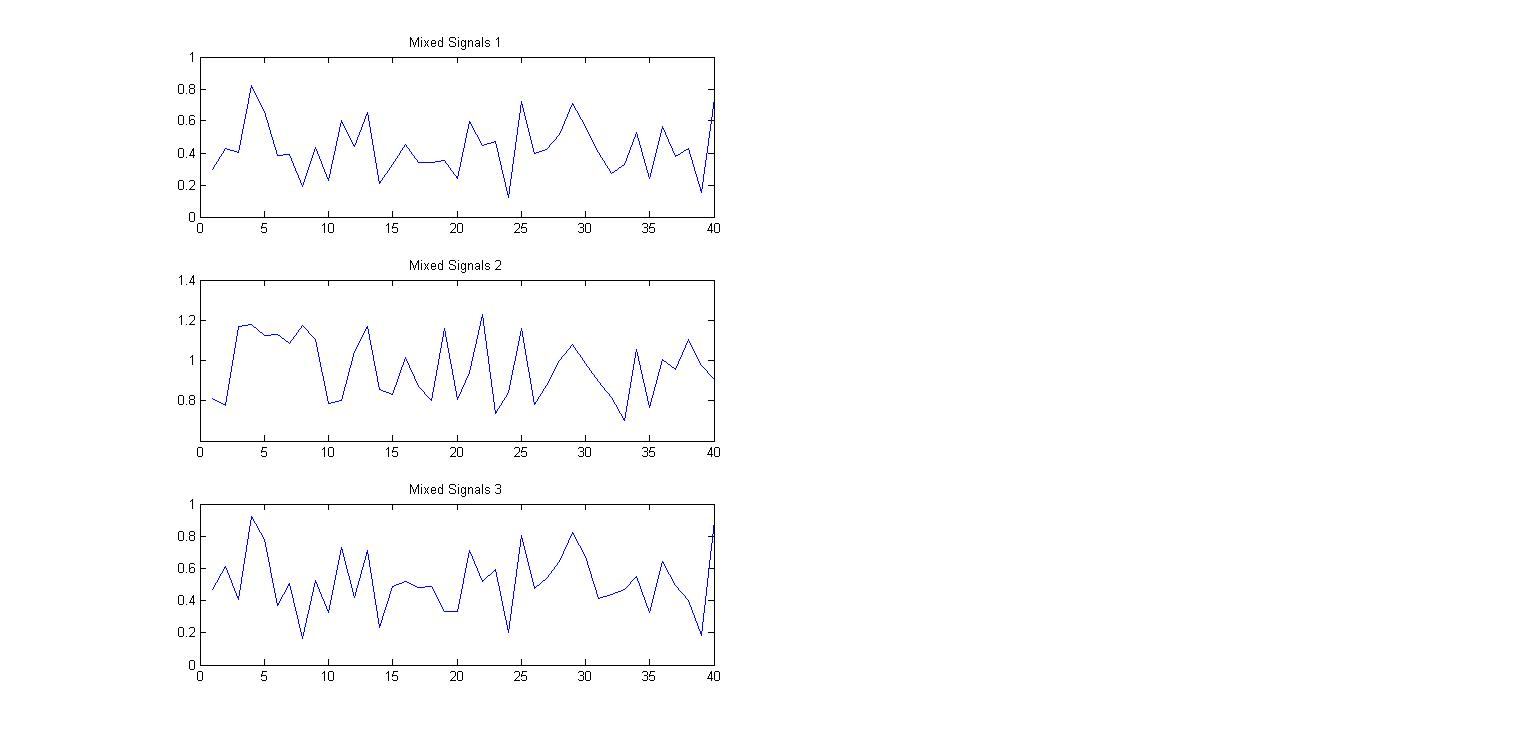
\includegraphics[width=\linewidth]{small_signal.jpg}
        Mixing Signals
    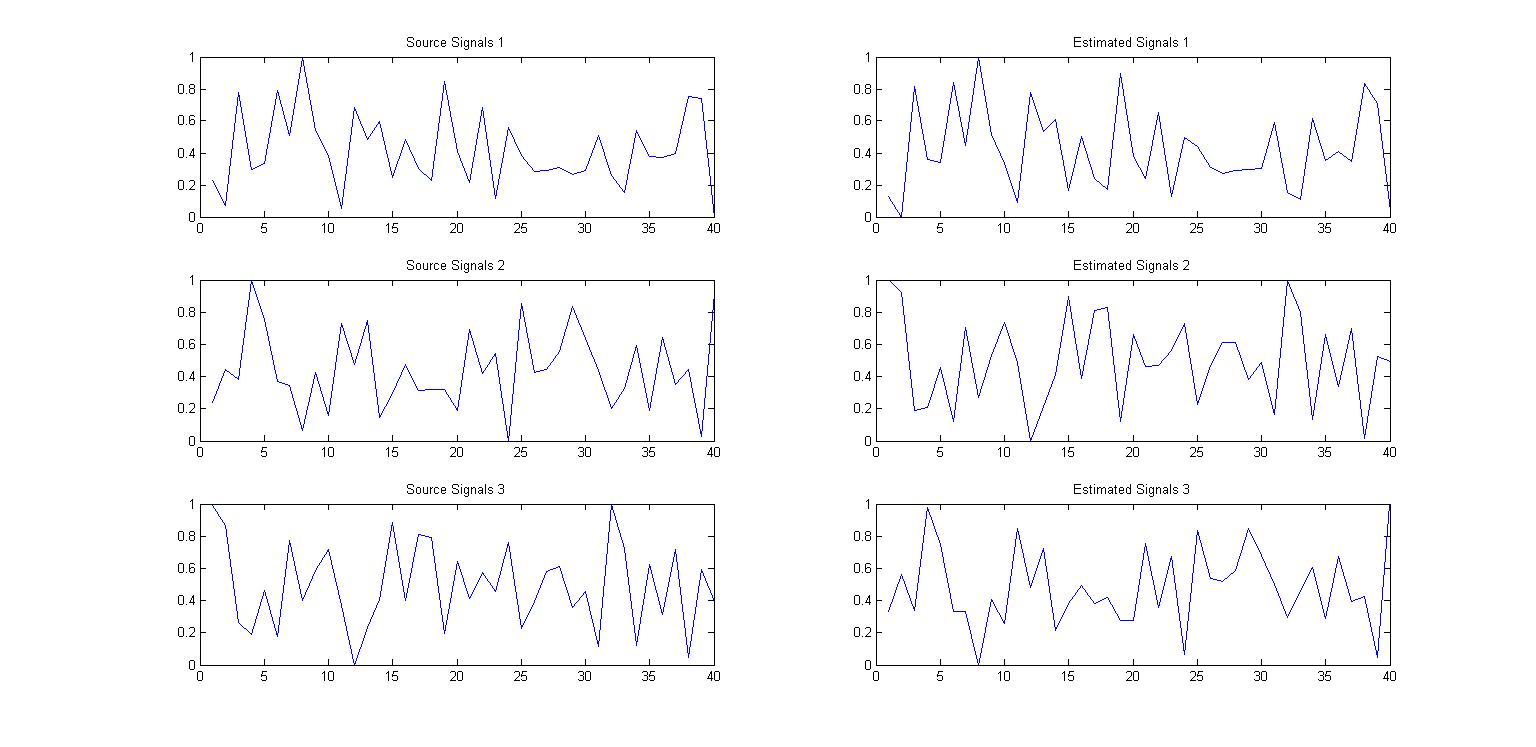
\includegraphics[width=\linewidth]{small_result.jpg}
        Origin and Recovered Signals. The Estimated Signals 2 and 3 are corresponding to Origin Signals 3 and 2.
\end{center}

\subsection{Large Dataset}
For the large dataset \textbf{sounds.mat}. My program cannot run very well. But I also do experiments about why the ICA doesn't work well. First, see my result for experiment of \textbf{sounds.mat}:

\begin{center}
    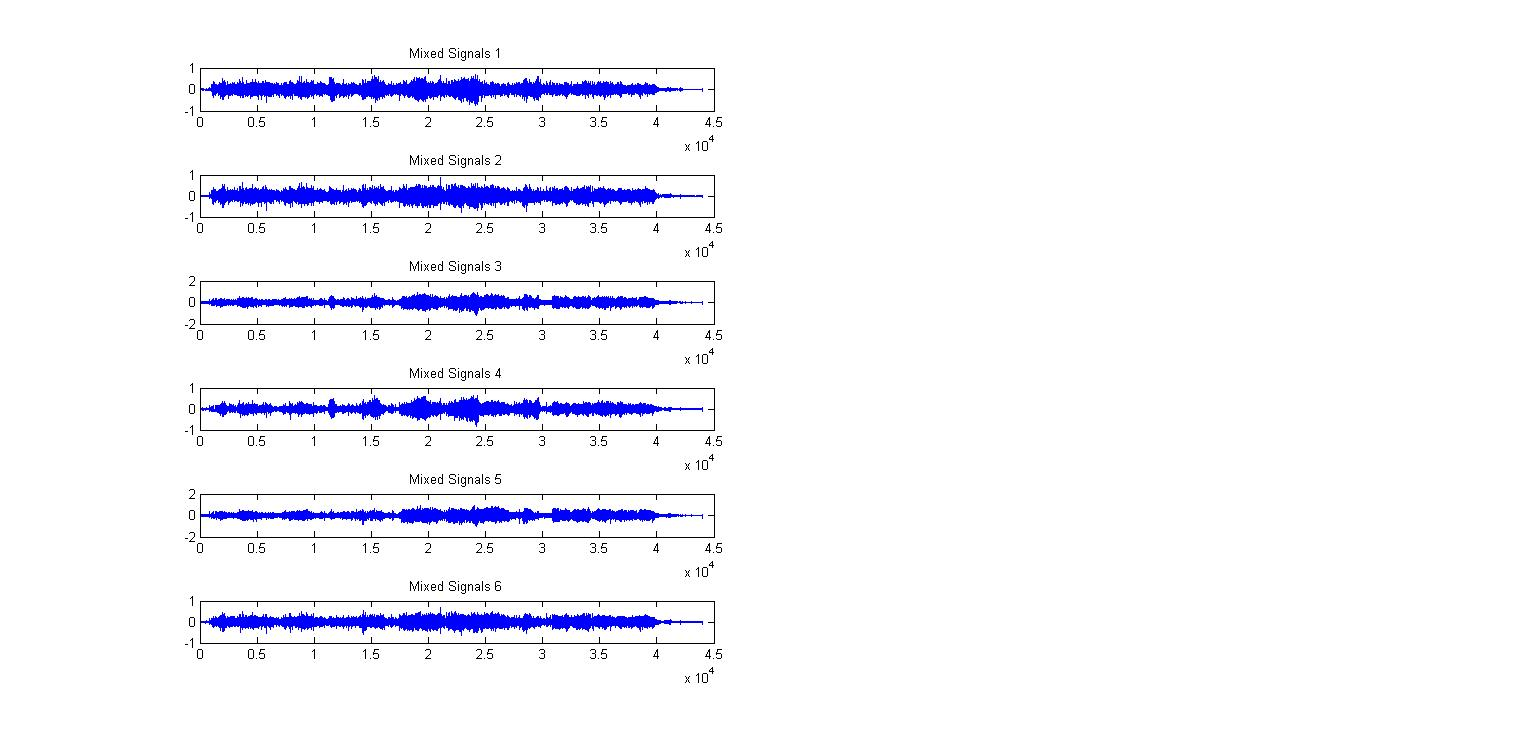
\includegraphics[width=\linewidth]{large_signal5.jpg}
        Mixing Signals of 5 Signals sounds.mat to 6 received signals
    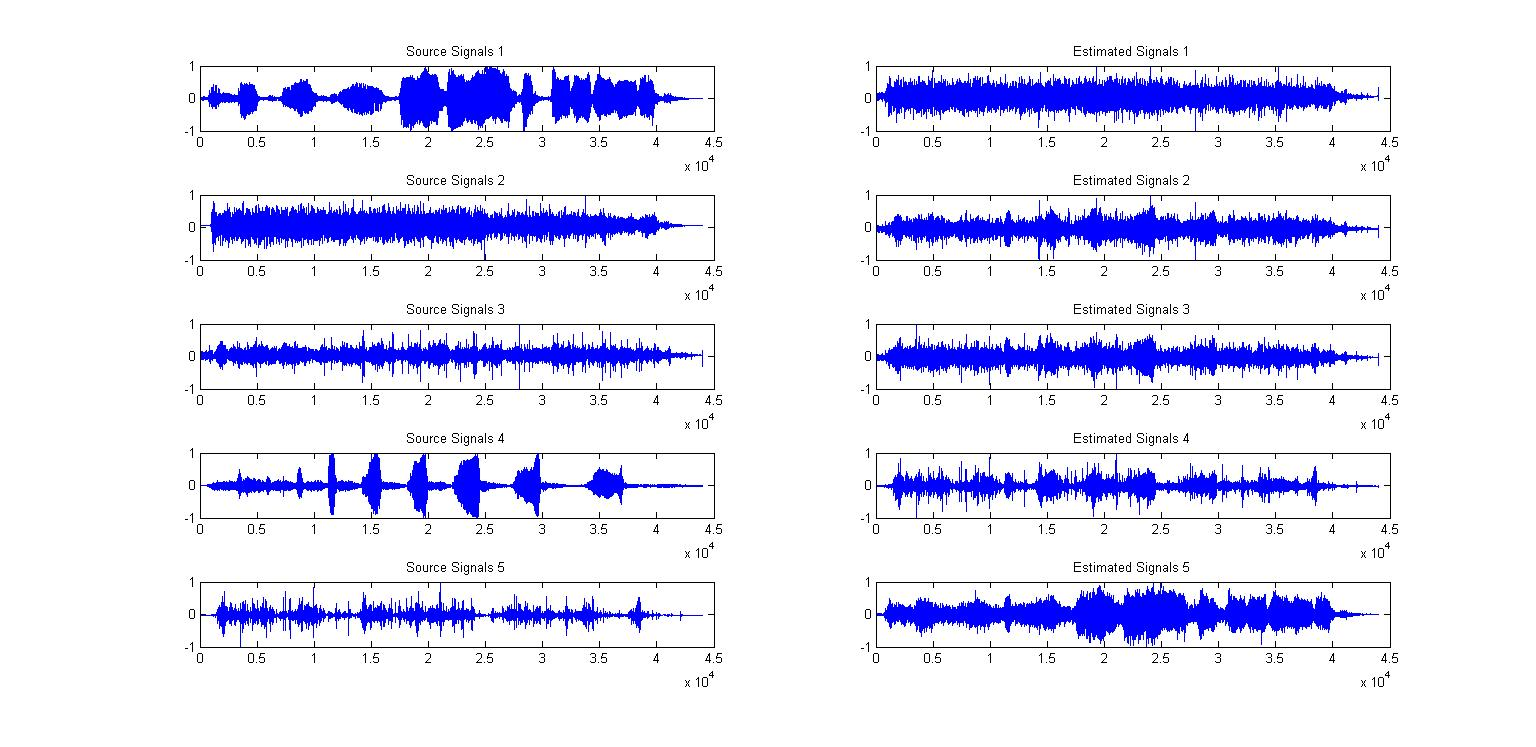
\includegraphics[width=\linewidth]{large_result5.jpg}
        Origin and Recovered Signals. 
    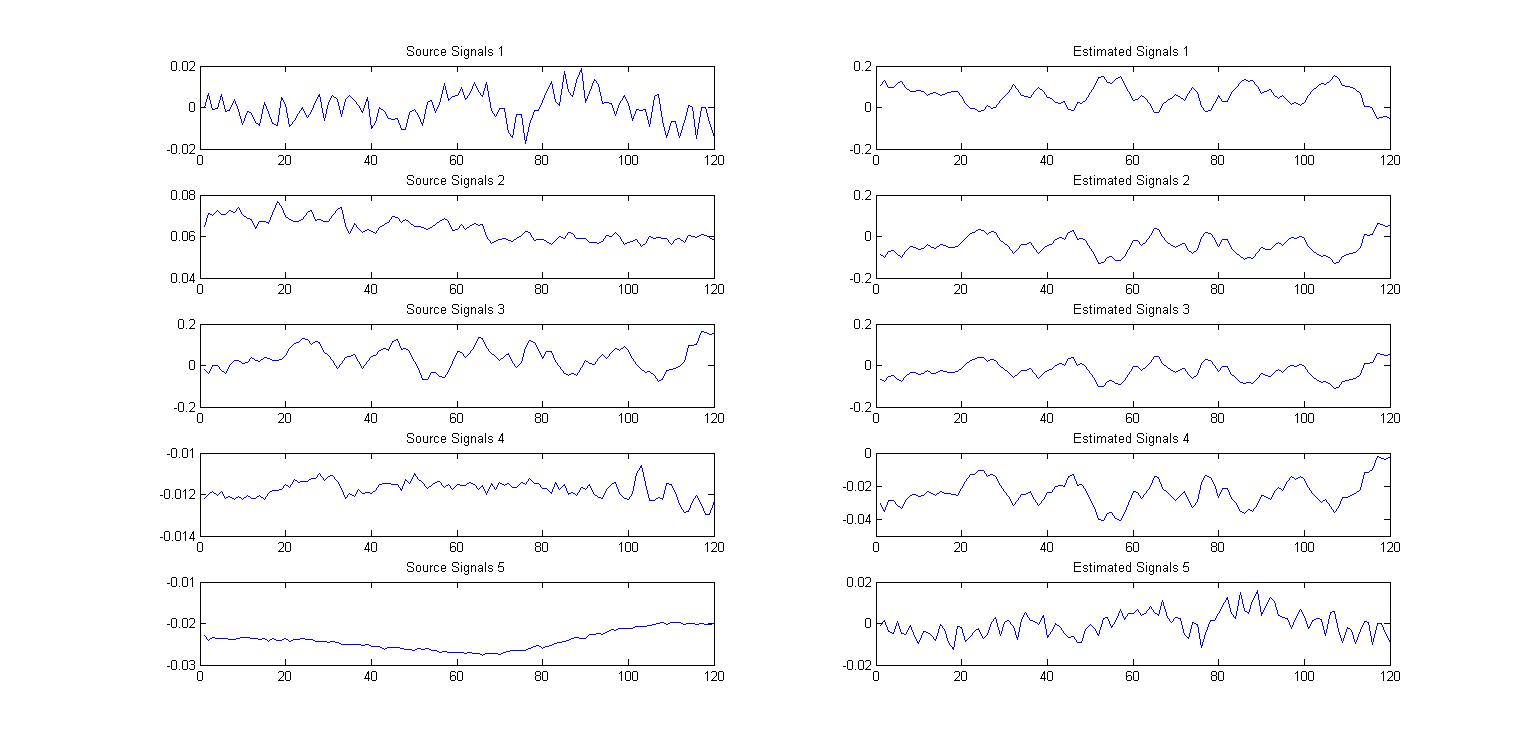
\includegraphics[width=\linewidth]{large_snap5.jpg}
        Snapshot of origin and recovered signals when $t <= 120$
\end{center}


The matrix sounds is $n * t$ matirx (number of signals multiplies time). Then I would think, is the ICA cannot work well for larger $n$ or larger $t$. I did experiment about just use first $n$ signals or first $t$ signals. My experiment result suggests that ICA can work well with larger $t$, smaller $n$. But it cannot work well with larger $n$:
\subsubsection{$n = 3, t = 44000$ }
\begin{center}
    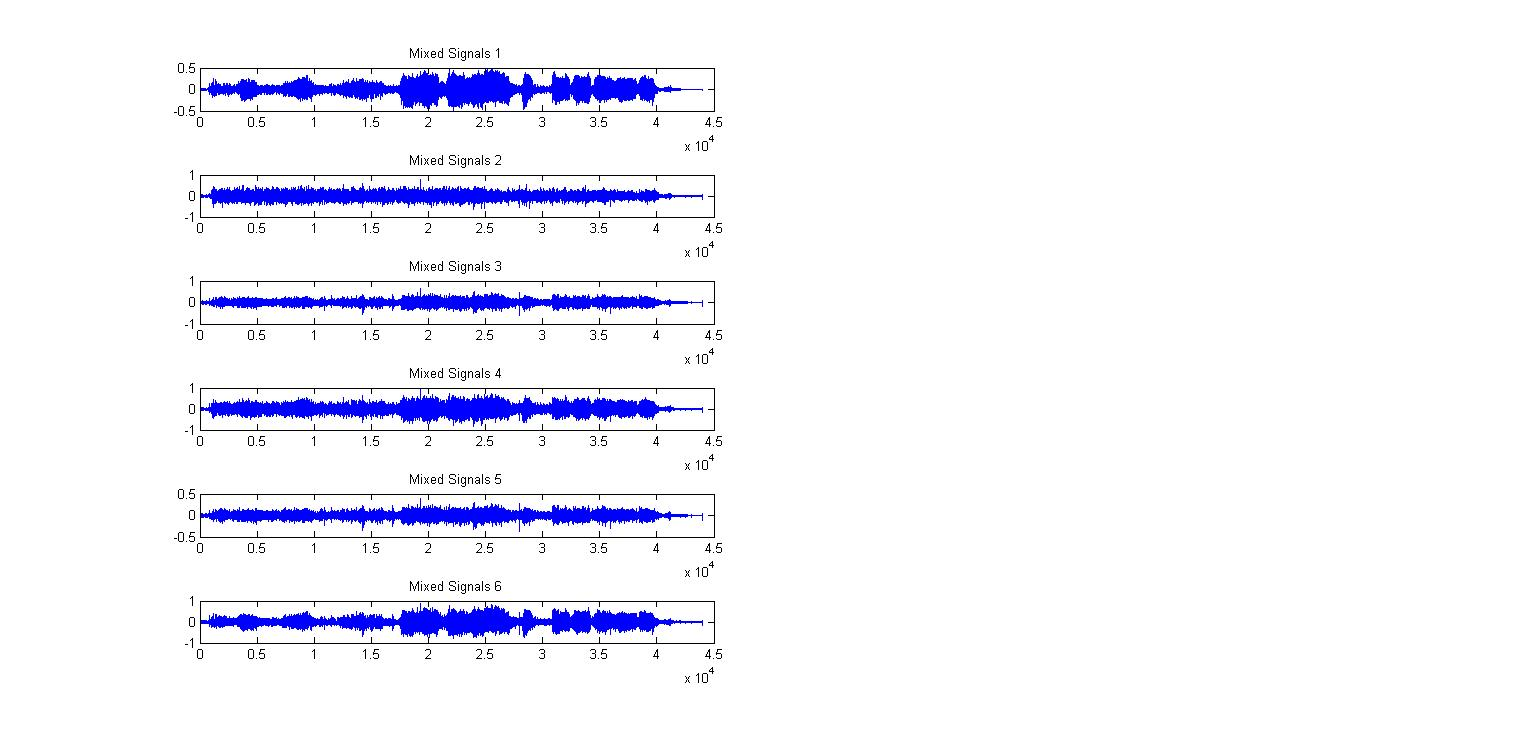
\includegraphics[width=\linewidth]{large_signal3.jpg}
        Mixing Signals of First 3 Signals sounds.mat
    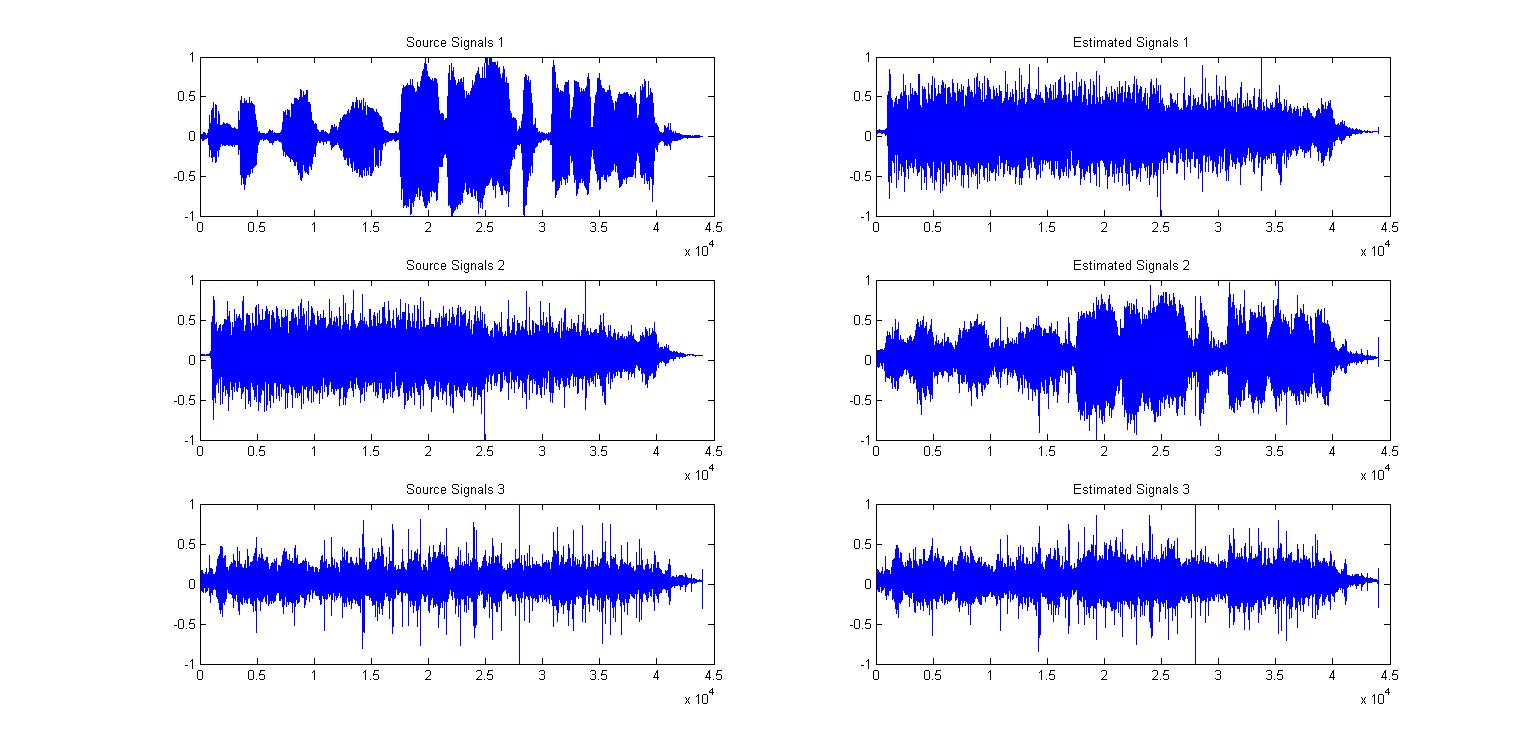
\includegraphics[width=\linewidth]{large_result3.jpg}
        Origin and Recovered Signals. The Estimated Signals 1 and 2 are corresponding to Origin Signals 2 and 1.
    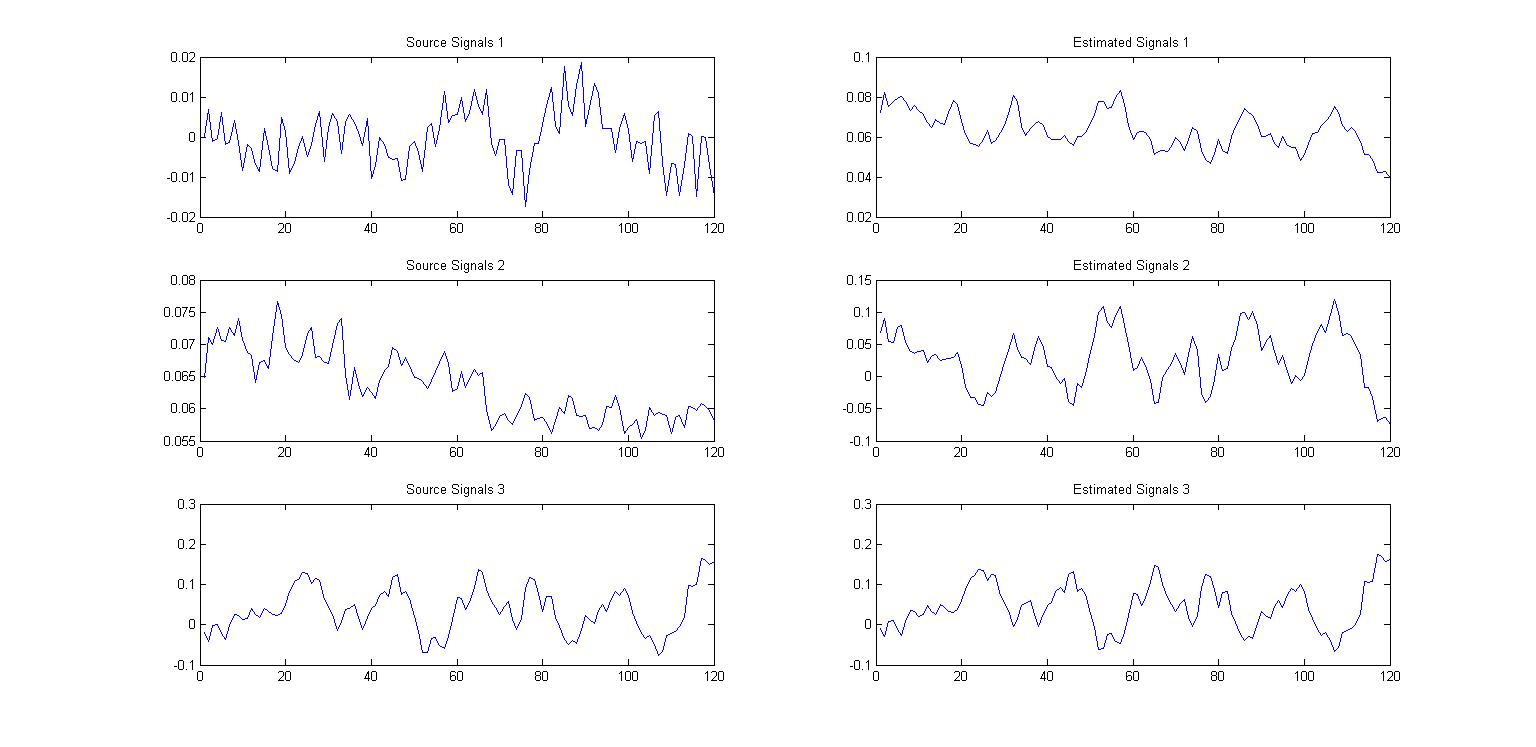
\includegraphics[width=\linewidth]{large_snap3.jpg}
        Snapshot of origin and recovered signals when $t <= 120$
\end{center}


\subsubsection{$t = 40, n = 6$}
\begin{center}
    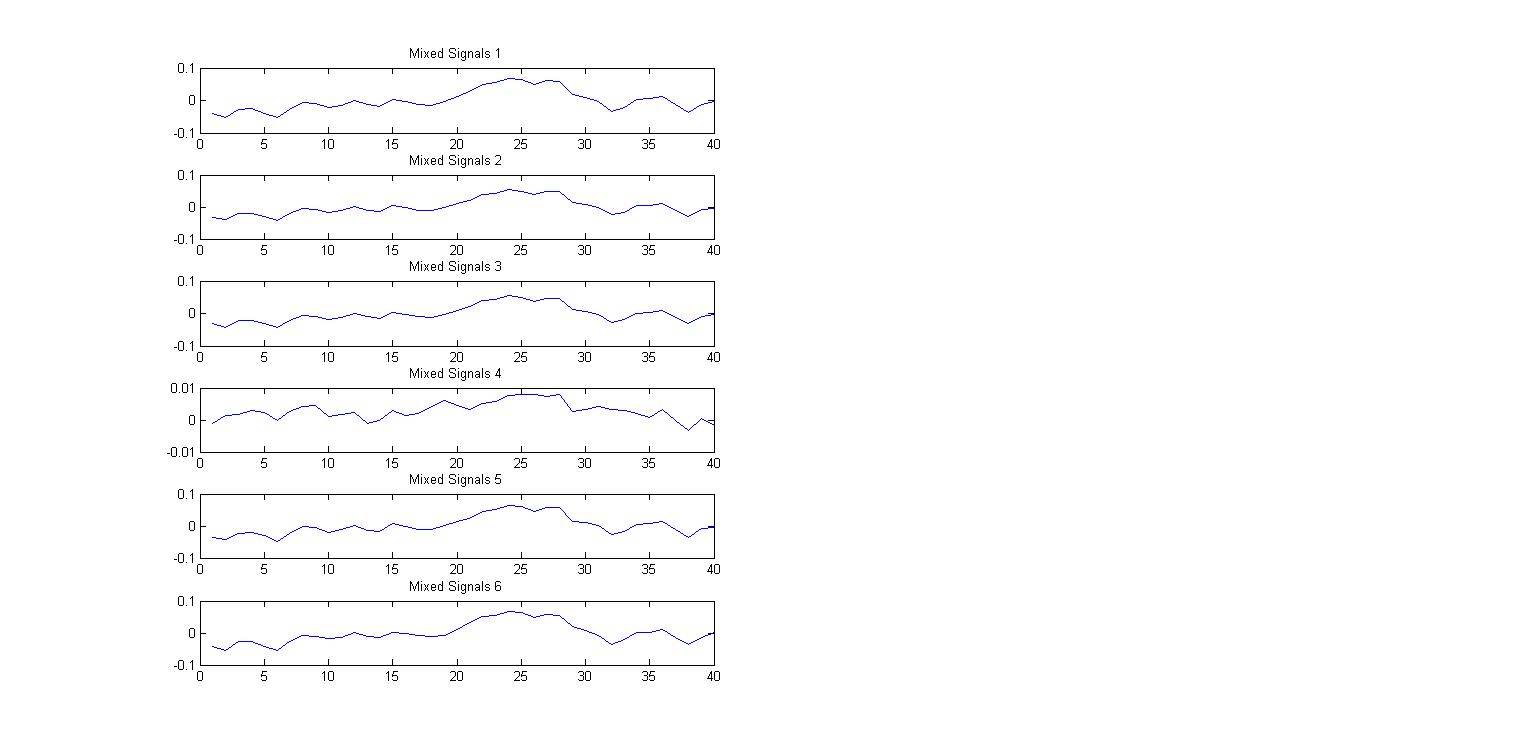
\includegraphics[width=\linewidth]{t40_signal.jpg}
        Mixing Signals of First 3 Signals sounds.mat
    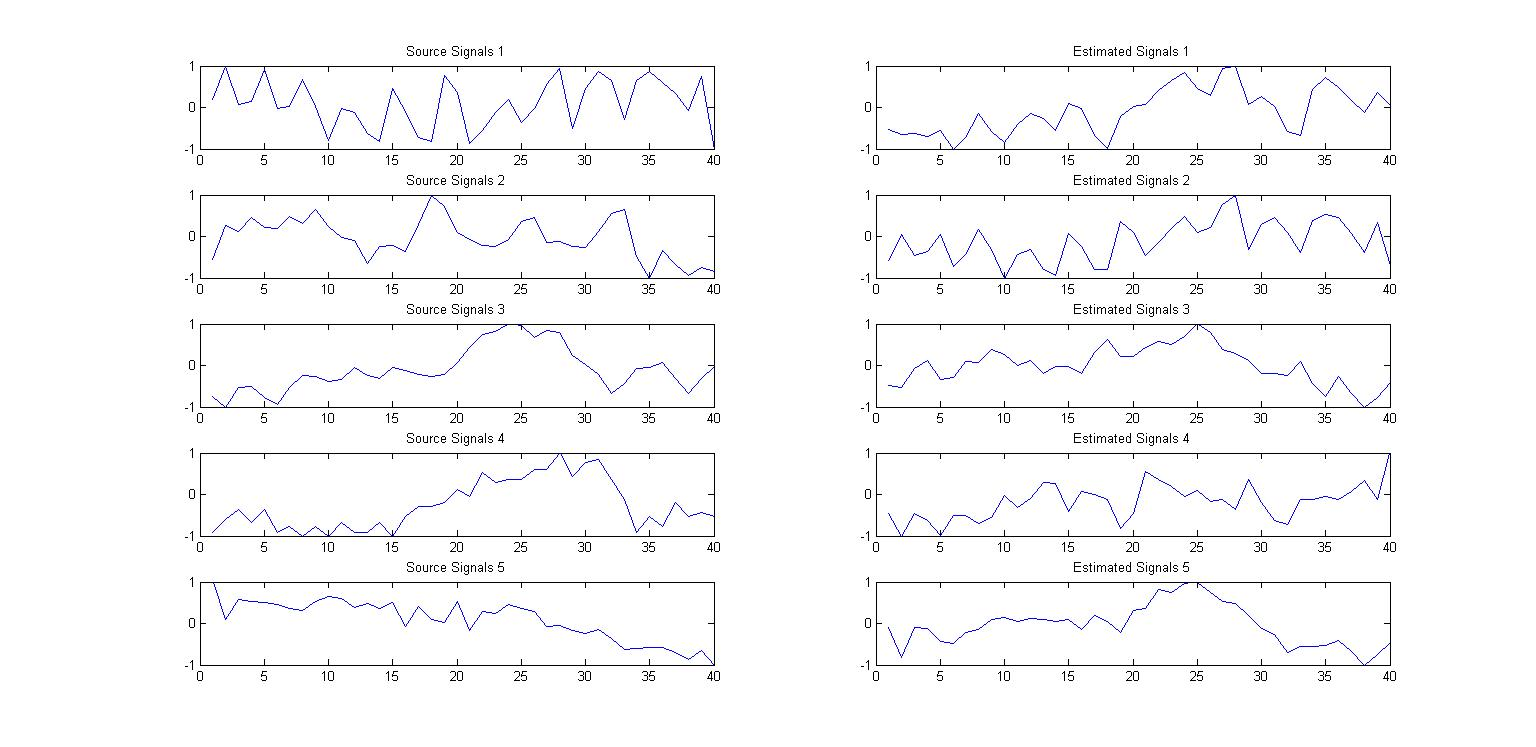
\includegraphics[width=\linewidth]{t40_result.jpg}
        Origin and Recovered Signals. 
\end{center}
From the experiment we can see ICA can work well with larger $t$, smaller $n$. But it cannot work well with larger $n$ even with small $t$.
\section{Conclusion}
In this assignment, I not only implemented the ICA algorithm, but 1, find another way to speed up converge in ICA. 2, find ICA cannot work well for larger number of signals, but can work for larger time.

\end{spacing}

%\end{CJK*}
\end{document}
